\section{Zuzanna Jarlaczyńska}
\label{zjarl}
I added a picture of a dog ( see Figure ~\ref{fig:dog})

\begin{figure}[htbp] 
    \centering
    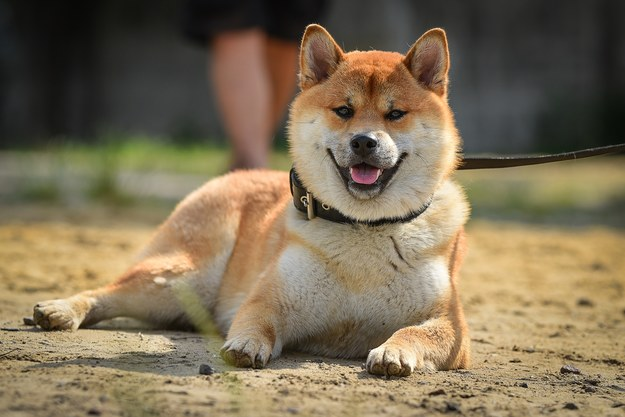
\includegraphics[width=0.5\textwidth, scale=5]{pictures/dog.jpeg}
\caption{This dog is cool.}
    \label{fig:dog}
\end{figure}

I added math equation: \[ (\sum_{i=1}^{n}x_{i}y_{i})^2 \leq (\sum_{i=1}^{n}x_{i}^2)(\sum_{i=1}^{n}y_{i}^2) \] 

\newpage

Table ~\ref{tab:trigonometry_table} represents trigonometry table. 

 \begin{table}[htbp]
 \centering
\begin{tabular}{
>{\columncolor[HTML]{E7E6E1}}c 
>{\columncolor[HTML]{FFFFFF}}c 
>{\columncolor[HTML]{FFFFFF}}c 
>{\columncolor[HTML]{FFFFFF}}c 
>{\columncolor[HTML]{FFFFFF}}c l}
\cellcolor[HTML]{E1DED2}\alpha & \cellcolor[HTML]{E1DED2}sin \alpha & \cellcolor[HTML]{E1DED2}cos \alpha & \cellcolor[HTML]{E1DED2}tg \alpha & \cellcolor[HTML]{E1DED2}ctg \alpha &  \\
0° & 0      & 1      & 0      & - &  \\
1° & 0.0175 & 0.9998 & 0.0175 & 57.29        &  \\
2° & 0.0349 & 0.9994 & 0.0349 & 28.6363      &  \\
3° & 0.0523 & 0.9986 & 0.0524 & 19.0811      &  \\
4° & 0.0698 & 0.9976 & 0.0699 & 14.3007      &  \\
5° & 0.0872 & 0.9962 & 0.0875 & 11.4301      & 

\end{tabular}
\label{tab:trigonometry_table}
\caption{This is a caption}
\end{table}

I added unordered list: \\
List of seasons
\begin{itemize}
    \item[$\blacksquare$] Spring
    \item[$\blacksquare$] Summer
    \item[$\blacksquare$] Autumn
    \item[$\blacksquare$] Winter 
\end{itemize}

I added ordered list: 
\begin{enumerate}
    \item Spring
    \item Summer
    \item Autumn
    \item Winter
\end{enumerate}
\begin{center}
\textbf{Short story}\\
\underline{\emph{Once upon a time}} there lived a dog in a forest. One day after a heavy meal. It was sleeping under a tree. After a while, there came a mouse and it started to play on the dog. Suddenly the dog got up with anger and looked for those who disturbed its nice sleep. Then it saw a small mouse standing trembling with fear. The dog jumped on it and started to kill it. The mouse requested the dog to forgive it. The dog felt pity and left it. The mouse ran away. \par
On another day, the dog was caught in a net by a hunter. The mouse came there and cut the net. Thus it escaped. There after, the mouse and the dog became friends. They lived happily in the forest afterwards. \par
\textit{The end}
\end{center}






